\subsubsection{Undicesimo periodo (2024/05/20 - 2024/05/29)}
\subsubsubsection{Planning}
In questo periodo, in vista della revisione $\textit{PB}_G$, si è cercato di terminare lo sviluppo dei requisiti funzionali dell'$\textit{MVP}_G$; di conseguenza, molte risorse sono state destinate ai ruoli dei Progettisti e dei Programmatori. \\
I membri del gruppo hanno portato avanti parallelamente lo sviluppo degli ultimi requisiti necessari per l'$\textit{MVP}_G$ redigendo il documento di Specifica Tecnica.
\subsubsubsubsection*{Attività pianificate}
Gli obiettivi posti per lo $\textit{sprint}_G$ sono stati i seguenti:
\begin{itemize}
    \item Effettuare degli incontri con il prof. Cardin per chiarire dei dubbi riguardanti la redazione del documento Specifica Tecnica;
    \item Effettuare degli incontri con il proponente per chiarire dei dubbi riguardanti la redazione del documento Specifica Tecnica e presentare lo stato di avanzamento del progetto.
    \item Aggiornare il documento di Analisi dei Requisiti;
    \item Progettare e codificare Sviluppare i requisiti obbligatori per l'$\textit{MVP}_G$.
\end{itemize}
\subsubsubsubsection*{Preventivo}
\begin{table}[H]
    \centering
\begin{spreadtab}{{tabular}{|c|c|c|c|c|c|c|c|}}
    \hline
    @\textbf{Membro} & @\textbf{Re} & @\textbf{Amm} & @\textbf{An} & @\textbf{Progr} & @\textbf{Proge} & @\textbf{Ve} & @\textbf{Totale} \\
    \hline
    @ Samuele V.   & 0          & 0          & 0         &11.5          & 1     & 10.58    & sum(b2:g2) \\
    @ Leonardo B.  & 2         & 0          & 0        & 8.5        & 0     & 6.5    & sum(b3:g3) \\
    @ Riccardo Z.  & 0          & 1.5          & 0          & 13         & 0     & 7.83  & sum(b4:g4) \\
    @ Davide B.    & 0          & 3         & 0       & 7      & 0     & 0.25     & sum(b5:g5) \\
    @ Michele Z.   & 0          & 0          & 0         & 3.5          & 0     & 2.5     & sum(b6:g6) \\
    @ Filippo T.   & 0          & 0          & 0         & 9          &  0    & 2     & sum(b7:g7) \\
    \hline
    @\textbf{Ore totali} & sum(b2:b7) & sum(c2:c7) & sum(d2:d7) & sum(e2:e7) & sum(f2:f7) & sum(g2:g7) &  sum(b8:g8)\\
    \hline
    @\textbf{Costo totale} & 30*b8 & 20*c8 & 25*d8 & 15*e8 & 25*f8 & 15*g8 & sum(b9:g9)\\
    \hline
\end{spreadtab}
    \caption{Preventivo orario ed economico parziale per l'undicesimo periodo, in base al ruolo}
    \label{tab:prev_rtb}
    \vspace{5mm}
    \textbf{Legenda:} \textit{Re} = Responsabile, \textit{Amm} = Amministratore, \textit{An} = Analista, \textit{Progr} = Programmatore, \textit{Proge} = Progettista, \textit{Ve} = Verificatore
\end{table}
\begin{figure}[H]
  \centering
  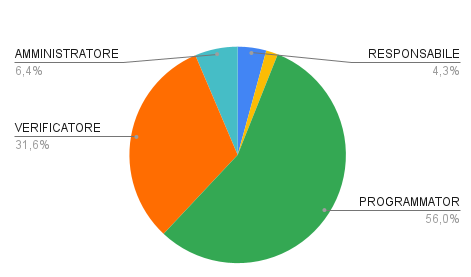
\includegraphics[width=0.6\linewidth]{grafici/11_periodo_torta.png}
  \caption{Ripartizione dei costi per ruolo nell'$11^\circ$ periodo}
        \vspace{5mm}
  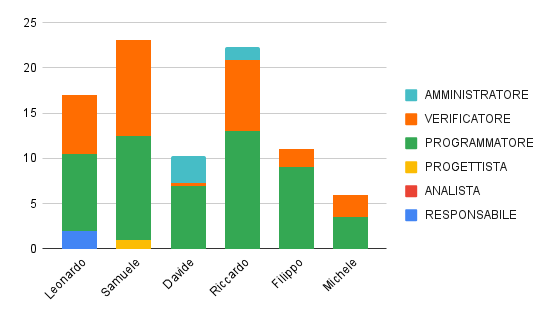
\includegraphics[width=0.7\linewidth]{grafici/11_periodo_istogramma.png}
  \caption{Ore preventivate per ciascuna persona nell'$11^\circ$ periodo}
\end{figure}
\subsubsubsection{Review}
Le attività preventivate sono state svolte con successo.
\subsubsubsubsection*{Attività svolte}
Le attività svolte in questo periodo sono state le seguenti:
\begin{itemize}
    \item Effettuato incontro con il proponente per discutere di dubbi riguardo al documento Specifica Tecnica; mostrato lo stato di avanzamento dei lavori.
    \item Effettuato incontro con il prof. Cardin per discutere di dubbi riguardanti il documento Specifica Tecnica.
\item Rivista la progettazione logica in seguito al $\textit{feedback}_G$ da parte del prof. Cardin.
\item Continuazione con la stesura del documento $\textit{Manuale Utente}_G$;
\item Completati i requisiti funzionali obbligatori;
\item Raggiunta la copertura dei $\textit{test}_G$ voluta dal proponente;
\item Implementato il $\textit{sistema}_G$ di notifica;
\item Effettuato incontro con il proponente per l'approvazione del $\textit{MVP}_G$ e ricevuta l'approvazione.
\end{itemize}
\subsubsubsubsection*{Consuntivo}
\begin{table}[H]
    \centering
\begin{spreadtab}{{tabular}{|c|c|c|c|c|c|c|c|}}
    \hline
    @\textbf{Membro} & @\textbf{Re} & @\textbf{Amm} & @\textbf{An} & @\textbf{Progr} & @\textbf{Proge} & @\textbf{Ve} & @\textbf{Totale} \\
    \hline
    @ Samuele V.   & 0          & 0          & 0         & 14          & 0.5     & 9.25     & sum(b2:g2) \\
    @ Leonardo B.  & 2.75         & 0          & 0        & 13.34        & 0     & 6.67    & sum(b3:g3) \\
    @ Riccardo Z.  & 0         & 1.5 & 0          & 14.17         & 0     & 5.83   & sum(b4:g4) \\
    @ Davide B.    & 0          & 6.75         & 0       & 11.5       & 0     & 0.5     & sum(b5:g5) \\
    @ Michele Z.   & 0          & 0          & 0         & 11.5          & 0     & 2.5     & sum(b6:g6) \\
    @ Filippo T.   & 0          & 0          & 0         & 5.5          & 0     & 0.83     & sum(b7:g7) \\
    \hline
    @\textbf{Ore totali} & sum(b2:b7) & sum(c2:c7) & sum(d2:d7) & sum(e2:e7) & sum(f2:f7) & sum(g2:g7) &  sum(b8:g8)\\
    \hline
    @\textbf{Costo totale} & 30*b8 & 20*c8 & 25*d8 & 15*e8 & 25*f8 & 15*g8 & sum(b9:g9)\\
    \hline
\end{spreadtab}
    \caption{Consuntivo orario ed economico parziale per l'undicesimo periodo, in base al ruolo}
    \label{tab:prev_rtb}
    \vspace{5mm}
    \textbf{Legenda:} \textit{Re} = Responsabile, \textit{Amm} = Amministratore, \textit{An} = Analista, \textit{Progr} = Programmatore, \textit{Proge} = Progettista, \textit{Ve} = Verificatore
\end{table}

\begin{comment}
\begin{figure}[H]
  \centering
  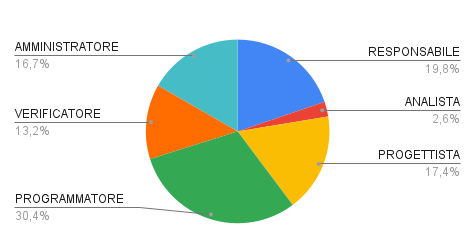
\includegraphics[width=0.6\linewidth]{grafici/10_periodo_torta.png}
  \caption{Ripartizione dei costi per ruolo nel $10^\circ$ periodo}
        \vspace{5mm}
  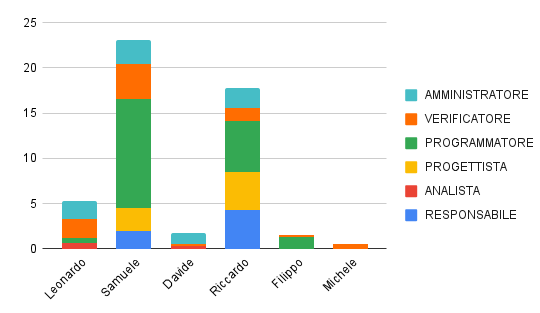
\includegraphics[width=0.7\linewidth]{grafici/10_periodo_istogramma.png}
  \caption{Ore preventivate per ciascuna persona nel $10^\circ$ periodo}
\end{figure}
\end{comment}

\begin{figure}[H]
  \centering
  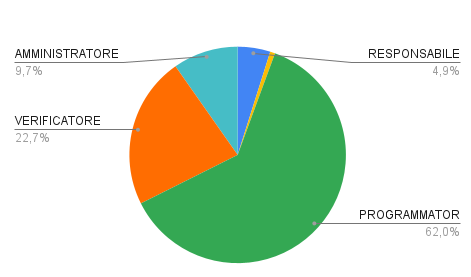
\includegraphics[width=0.6\linewidth]{grafici/11_periodo_torta_consuntivo.png}
  \caption{Consuntivo della ripartizione dei costi per ruolo nell'$11^\circ$ periodo}
        \vspace{5mm}
  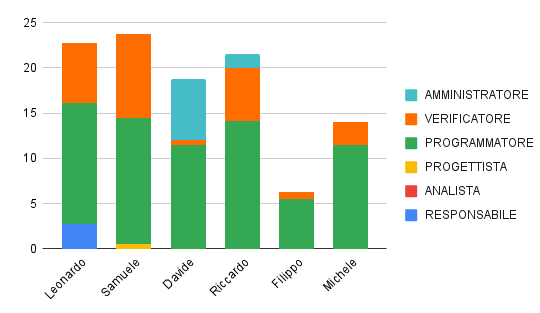
\includegraphics[width=0.7\linewidth]{grafici/11_periodo_instogramma_consuntivo.png}
  \caption{Ore eseguite per ciascuna persona nell'$11^\circ$ periodo}
\end{figure}

\subsubsubsection{Retrospective}
\paragraph*{Gestione dei Rischi}
I $\textit{rischi}_G$ affrontati durante questo periodo sono stati i seguenti:
\begin{itemize}
\item \nameref{ro:2}: la limitata disponibilità di alcuni membri del team ha determinato un rallentamento previsto nello $\textit{sprint}_G$.
\begin{itemize}
\item \textbf{Esito della mitigazione}: una redistribuzione di alcune attività ha comunque permesso di completare lo $\textit{sprint}_G$ e implementare tutte le funzionalità rimanenti.
\item \textbf{Impatto}: La redistribuzione ha causato un maggiore squilibrio nelle ore individuali lavorate dai membri del gruppo.
\end{itemize}
\item \nameref{ro:5}: la scarsa esperienza nella progettazione e nel testing ha comportato un rallentamento previsto nello $\textit{sprint}_G$.
\begin{itemize}
\item \textbf{Esito della mitigazione}: le attività di studio individuale, le discussioni di gruppo e gli incontri frequenti con il proponente e il prof. Cardin sono stati elementi chiave per mitigare questo rischio. In particolare, per ogni risultato ottenuto in fase di testing e progettazione, è stata fornita una dimostrazione al proponente, ottenendo un riscontro tempestivo; i progressi nella stesura del documento Specifica Tecnica sono stati mostrati al prof. Cardin, che ha fornito $\textit{feedback}_G$ al gruppo.
\item \textbf{Impatto}: in ambito progettuale, sono stati chiariti alcuni dubbi relativi al documento Specifica Tecnica.
\end{itemize}
\end{itemize}
\paragraph*{Considerazioni e pianificazione futura}
\begin{itemize}
    \item L'incontro con il prof. Cardin ha evidenziato i problemi dell'$\textit{architettura}_G$ logica del prodotto. Infatti il gruppo ha compreso che si doveva modificare l'$\textit{architettura}_G$ logica suddividendola da quella di $\textit{deployment}_G$.
    \item Nel periodo successivo si dovrà sistemare il documento di Specifica Tecnica per sostenere la revisione $\textit{PB}_G$ con il prof. Cardin.
\end{itemize}
 